\providecommand{\main}{../../..}
\documentclass[\main/main.tex]{subfiles}
\begin{document}
\chapter{Disuguaglianze forti valide}
Per disuguaglianze\textit{forti} si intende una disuguaglianza che porta ad una formulazione \textit{migliore}. Purtroppo, spesso, descrivere famiglie di disuguaglianze forti risulta piuttosto complesso ed il problema di separazione che vanno a porre altrettanto, che talvolta risulta essere \textbf{NP-hard}.

Queste disuguaglianze vengono usate per risolvere problemi grandi e/o complessi integrandole in un modello branch-and-bound, che nello specifico viene chiamato \textbf{branch-and-cut}.

\section{Definizioni preliminari}
\subsection{Definizioni sulle disuguaglianze}
\begin{figure}
    \begin{subfigure}{0.49\textwidth}
        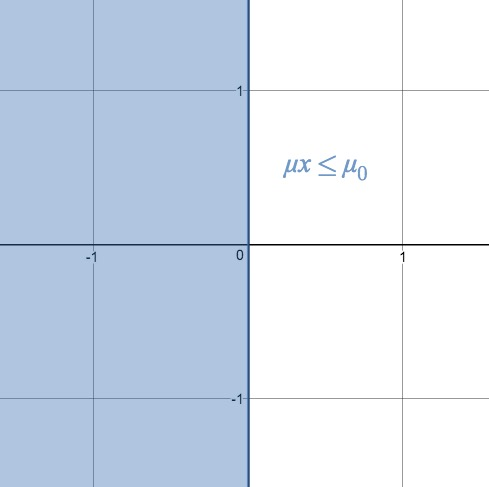
\includegraphics[width=0.4\textwidth]{strong/equiv_1}
    \end{subfigure}
    \begin{subfigure}{0.49\textwidth}
        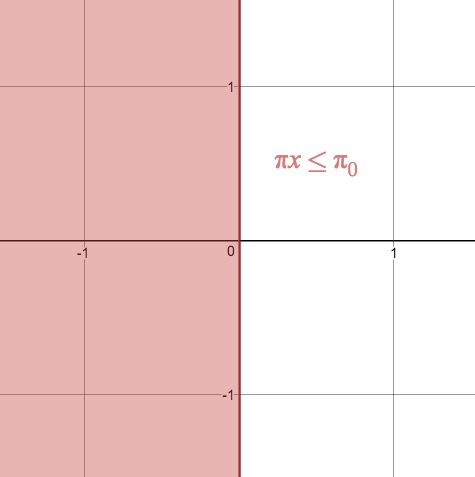
\includegraphics[width=0.4\textwidth]{strong/equiv_2}
    \end{subfigure}
    \caption{Disuguaglianze equivalenti}\label{ineqequivalent}
\end{figure}
\begin{definition}[Disuguaglianze equivalenti]
    Due disuguaglianze \(\bm{\pi}\bmx \leq \bm{\pi}_{0}\) e \(\bm{\mu}\bmx \leq \bm{\mu}_{0}\) valide per \(P\subseteq\R^n_+\) sono \textbf{equivalenti} (\ref{ineqequivalent}) se:
    \[
        \exists \lambda>0: \bm{\pi} = \lambda\bm{\mu} \quad \land \bm{\pi}_{0} = \lambda\bm{\mu}_{0}
    \]\end{definition}
\begin{figure}
    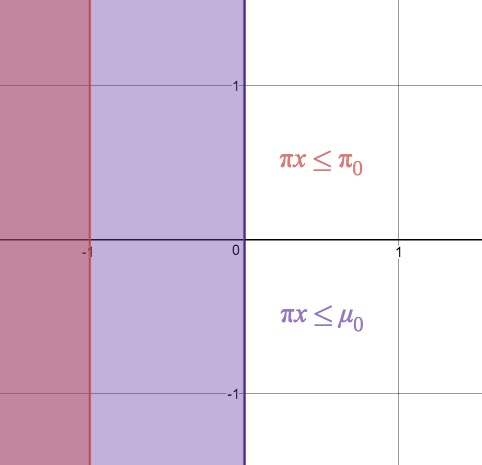
\includegraphics[width=0.25\textwidth]{strong/domin}
    \caption{Disuguaglianze dominanti e ridondanti}\label{ineqdomin}
\end{figure}
\begin{definition}[Disuguaglianze dominanti]
    Se due disuguaglianze \(\Pi: \bm{\pi}\bmx \leq \bm{\pi}_{0}\) e \(M:\bm{\mu}\bmx \leq \bm{\mu}_{0}\) sono valide per \(P\subseteq\R^n_+\), si dice che \(\Pi \) \textbf{domina} \(M\)~\ref{ineqdomin} se esse non sono equivalenti e:
    \[
        \exists \lambda>0: \bm{\pi} \geq \lambda\mu \quad \bm{\pi}_0 \leq \lambda\mu_0
    \]    Il poliedro descritto dalla disuguaglianza dominante è contenuto nel poliedro della disuguaglianza dominata.
\end{definition}
\begin{definition}[Disuguaglianze ridondante]
    Una disuguaglianza valida \(\Pi: \bm{\pi}\bmx \leq \bm{\pi}_{0}\) è detta \textbf{ridondante} nella descrizione di \(\matr{P}\) se esistono una o più disuguaglianze valide su \(\matr{P}\) che la dominano.

    Una disuguaglianza non ridondante è detta \textbf{unica}.
\end{definition}

Dove non è possibile ottenere una descrizione esplicita di \(P = \text{conv}(X)\), come nel caso di problemi NP-hard (a meno che \(\mathcal{P}=\mathcal{NP}\)), identificare equazioni ridondanti può risultare molto difficile.

\subsection{Definizioni sui poliedri}
\begin{definition}[Poliedro dimensionalmente completo]
    Un poliedro \(P\subseteq\R^n\) che contiene \(n\) direzioni linearmente indipendenti è detto \textbf{dimensionalmente completo}.
\end{definition}

\begin{proposition}[Non-esistenza di equivalenze valide per poliedri dimensionalmente completi]
    Se \(\matr{P}\) è un poliedro dimensionalmente completo, allora non esiste un'equazione \(\bma\bmx = \bmb \) che sia valida \(\forall \bmx \in P\).
\end{proposition}

\begin{theorem}[Descrizione minimale unica di un poliedro dimensionalmente completo]
    Se \(\matr{P}\) è un poliedro dimensionalmente completo, esso possiede una descrizione minimale unica:
    \[
        P = \crl{\bmx \in \R^n: a_i\bmx \leq b_i \quad \forall i \in [1, \ldots, m]}
    \]    dove ogni disuguaglianze è unica.
\end{theorem}
\begin{definition}[Punti indipendenti affini]
    Un insieme di punti \(\crl{\bmx_1, \ldots, \bmx_k} \in \crl{\R^n}^k\) sono detti \textbf{indipendenti affini} se le \(k-1\) direzioni \(\bmx_2 - \bmx_1, \ldots, \bmx_k - \bmx_1\) sono linearmente indipendenti.
\end{definition}
\begin{definition}[Dimensione di un poliedro]
    Con dimensione di un poliedro \(P\subseteq \R^n\), è pari a \(\dim(P) = \#\crl{\bmx_{\text{ind. aff.}} \in P} -1\), cioè contiene \(n\) direzioni linearmente indipendenti.
\end{definition}
\begin{definition}[Faccia di poliedro]
    \(F\) definisce una \textbf{faccia} di un poliedro \(\matr{P}\) se \(F = \crl{\bmx \in P: \bm{\pi}\bmx = \bm{\pi}_0}\) per una disuguaglianza valida \(\bm{\pi}\bmx = \bm{\pi}_0\) di \(\matr{P}\).

    Una faccia di un poliedro è a sua volta un poliedro ed il numero di facce di un poliedro è finito.
\end{definition}
\begin{definition}[Sfaccettatura di poliedro]
    \(F\) definisce una \textbf{sfaccettatura} di un poliedro \(\matr{P}\) se è una faccia di \(\matr{P}\) e \(\dim(F) = \dim(P) -1\).
\end{definition}
\begin{definition}[Disuguaglianze rappresentante (o definente) una faccia di poliedro]
    Data una \textbf{faccia} \(F\) di un poliedro \(\matr{P}\) definita come \(F = \crl{\bmx \in P: \bm{\pi}\bmx = \bm{\pi}_0}\), la disuguaglianza che la caratterizza è detta \textbf{rappresentante} la faccia.
\end{definition}

\begin{proposition}[Disuguaglianza necessaria]
    Se il poliedro \(\matr{P}\) è dimensionalmente completo, una disuguaglianza valida \(\bm{\pi}\bmx \leq \bm{\pi}_0\) è \textbf{necessaria} nella descrizione di \(\matr{P}\) se e solo se rappresenta una \textbf{sfaccettatura} di \(\matr{P}\).

    Ciò significa che una disuguaglianza definisce una sfaccettatura di \(\matr{P}\) se e solo se esistono \(n\) punti indipendenti \(\bmx \in P\) che ne soddisfano la forma in uguaglianza: questi punti saranno quindi posizionati su un generico iperpiano \(\bm{\mu}\bmx = \bm{\mu}_0\).

    \[
        \sum_{j=1}^n \mu_j\bmx_{jk} = \mu_0 \quad \forall k
    \]
    Se l'unica soluzione ammissibile è per \((\mu, \mu_0) = \lambda (\pi, \pi_0) \quad \lambda \neq 0\) allora \(\bm{\pi}\bmx \leq \bm{\pi}_0\) è rappresenta una sfaccettatura ed è quindi \textbf{necessaria}.
\end{proposition}

\section{Dimostrare che un poliedro descrive un insieme convesso}
Esistono diversi approcci per mostrare che un poliedro \(P = \crl{\bmx \in \R^n: \matr{A}\bmx \leq \bmb}\) descrive \(\conv(X)\):

\begin{enumerate}
    \item Mostrare che la matrice \(\matr{A}\), o la coppia \(\matr{A}, \bmb \) ha una struttura particolare che garantisce che \(P = \conv(X)\).
    \item Mostrare che i punti \(\crl{\bmx, \bmy} \in P\) con \(\bmy \) frazionario non sono \textbf{vertici} di \(\matr{P}\).
    \item Mostrare che per qualsiasi punto \(\bmc \in \R^n\), il programma lineare \(z_{LP} = \max\crl{\bmc\bmx: \matr{A}\bmx \leq \bmb}\) ha una soluzione ottima \(\bmxo \in X\).
    \item Mostrare che \(\forall \bmc \in \R^n \) esiste un punto \(\bmxo \in X\) e una soluzione ammissibile \(\bmuo \) del problema duale \(\w_{LP} = \min\crl{\bmu\bmb: \bmu \matr{A} = \bmc, \bmu \geq 0}\) con \(\bmc\bmxo = \bmuo\bmb \).
    \item Mostrare che se \(\bm{\pi}\bmx \leq \bm{\pi}_0\) rappresenta una sfaccettatura di \(\conv(X)\), allora deve essere identica a una delle disuguaglianze che rappresentano \(\matr{P}\).
    \item Mostrare che \(\forall \bmc \in \R^n, \bmc \neq 0 \) l'insieme delle soluzioni ottime di \(\max\crl{\bmc\bmx: \bmx \in X}\) è contenuto in una delle disuguaglianze rappresentanti \(\matr{P}\).
    \item Verificare che \(\bmb \in \Z^n\) e che \(\forall \bmc \in \Z^n\), il valore ottimo del problema duale \(\w_{LP}\) ha valore intero.
\end{enumerate}

\clearpage
\section{Cover Inequalities}
Consideriamo il set di possibili soluzioni di un problema dello zaino a pesi e peso massimo strettamente positivi \(X = \crl{\bmx \in B^n: \sum_{i=1}^n \bmx_i a_i \leq b}\).

\begin{definition}[Cover]
    Un set \(S\subseteq N\) è una \textbf{cover} se \(\sum_{i\in S} a_i > b\). Una cover è detta \textbf{minimale} se \(C\bs\crl{j}\) non è una cover per nessun \(j \in C\).

    Il \textbf{vettore di incidenza associato} alla cover \(\bmx^C\) \textbf{non appartiene} alla regione ammissibile definita da \(X\).

    Se un set \(T\subseteq N\) contiene una cover \(C\), allora anche \(T\) è una cover.
\end{definition}

\begin{proposition}[Validità di una cover inequality]
    Se \(C\subseteq N\) è una cover per \(X\), allora la cover inequality
    \[
        \sum_{j \in C} x_j \leq \abs{C} -1
    \]    È valida per \(X\)
\end{proposition}

\section{Irrobustire una cover inequality}
\begin{proposition}
Se \(C\) è una cover per \(X\), la cover inequality estesa\[
    \sum_{j \in E(C)} x_j \leq \abs{C} -1
\]è valida per \(X\), dove \(E(C) = C \cup \crl{j: a_j \geq a_i \quad \forall i \in C}\)
\end{proposition}
\clearpage
\section{Sollevare le cover inequalities}
In generale il problema risulta essere trovare il miglior valore possibile di un peso \(\a_j, j \in N\bs C\) in modo tale che la disuguaglianza
\[
    \sum_{j \in C}x_j + \sum_{j \in N\bs C} \a_j \bmx_j \leq \abs{C} -1
\]sia valida in \(X\).

La procedura di sollevamento delle cover inequalities è un metodo per produrre questo set di valori.

Siano \(j_1, \ldots, j_r\) un insieme ordinato di \(N\bs C\) e sia \(t\) uno scalare inizialmente di valore pari a \(1\). Si inizia dalla migliore uguaglianza identificata sino ad ora:
\[
    \sum_{j \in C}x_j + \sum_{i =1}^{t-1} \a_{j_i} \bmx_{j_i} \leq \abs{C} -1
\]
E si procede ad identificare il massimo valore di \(\a_{j_i}\) per cui essa risulta essere valida risolvendo il seguente problema dello zaino:

\begin{figure}
    \begin{align*}
         \xi_t = \max \sum_{j \in C}x_j + \sum_{i =1}^{t-1} \a_{j_i} \bmx_{j_i}\\
        \sum_{j \in C}x_j + \sum_{i =1}^{t-1} a_{j_i} \bmx_{j_i} &\leq b - a_{j_t}\\
        x \in \crl{0,1}^{\abs{C}+t-1}
    \end{align*}
    \caption{Problema dello zaino per il sollevamento delle cover inequalities}
\end{figure}

Si inizializza \(\a_{j_t} = \abs{C} -1 - \xi_t\) e si interrompe l'iterazione quando \(t = r\).

\section{Separazione delle cover inequalities}
Sia \(\mathcal{F}\) la famiglia delle cover inequalities per \(X\) e procediamo ad esaminare il problema della separazione su questa famiglia. Dato un punto non-intero \(\bmxo \in {[0,1]}^n\) vogliamo verificare se esso soddisfi o meno tutte le cover inequalities. Questo può essere formalizzato come:
\[
    \sum_{j \in C} (1-x_j) \geq 1
\]
La domanda che ci poniamo quindi è la seguente: esiste un set \(C \subseteq N\) tale che \(\sum_{j\in X}a_j>b\) per cui \(\sum_{j \in C} (1-x_j^*) <1\)?

Espresso in termini formali, la seguente disequazione è valida?
\[
    \xi = \min\crl{\sum_{j\in N}(1-x_j^*)z_j: \sum_{j\in N} a_j z_j > b, z \in B^n} < 1
\]
\begin{theorem}
\begin{enumerate}
    \item Se \(\xi\geq 1\) allora \(x^*\) soddisfa tutte le cover inequalities.
    \item Se \(\xi\leq 1\) con come soluzione ottimale \(z^R\), allora la cover inequality \(\sum_{j \in R} x_j \leq \abs{R} -1 \) taglia il punto \(\bmxo \) di un valore pari \(1-\xi \).
\end{enumerate}
\end{theorem}

\clearpage
\section{Disuguaglianze cover per i flussi}
\begin{definition}[Cover generalizzata]
    Un insieme \(C = C_1 \cup C_2\) con \(C_1 \subseteq N_1, C_2 \subseteq N_2\) è una \textbf{cover generalizzata} per \(X\) se:
    \[
        \sum_{j \in C_1} a_j - \sum_{j \in C_2} a_j = b + \lambda, \quad \lambda>0
    \]    Il termine \(\lambda \) è chiamato \textbf{eccesso della cover}
\end{definition}

\begin{proposition}
    La disuguaglianza cover di flusso:
    \[
        \sum_{j \in C_1} x_j + \sum_{j \in C_1} \rnd{a_j - \lambda}^+\rnd{1-y_j} \leq b + \sum_{j \in C_2} a_j + \lambda \sum_{j \in L_2}y_j + \sum_{j \in N_2 \bs \crl{C_2 \cup L_2}}x_j
    \]    È valida per \(X\), dove \(L_2 \subseteq N_2 \bs C_2\).
\end{proposition}

\subsection{Separazione per le disuguaglianze cover per i flussi}
Se si procede con l'assunzione che \(x_j = a_j y_j\), \(a_j \geq \lambda \quad \forall j \in C_1\) e che \(L_2 = N_2 \bs C_2\), la disuguaglianza cover per i flussi diviene:
\begin{align*}
    \sum_{j \in C_1} a_j y_j + \sum_{j \in C_1} \rnd{a_j - \lambda}^+\rnd{1-y_j} &\leq b + \sum_{j \in C_2} a_j + \lambda \sum_{j \in L_2}y_j + \sum_{j \in N_2 \bs \crl{C_2 \cup L_2}}a_j y_j\\
    \sum_{j \in C_1} a_j - \lambda\sum_{j \in C_1} \rnd{1-y_j} &\leq b + \sum_{j \in C_2} a_j + \lambda\sum_{j \in N_2 \bs C_2} y_j\\
    \sum_{j \in C_1} \rnd{1-y_j} + \sum_{j \in N_2 \bs C_2} y_j &\geq 1\\
    \sum_{j \in C_1} \rnd{1-y_j} - \sum_{j \in C_2} y_j &\geq 1 - \sum_{j \in N_2} y_j\\
\end{align*}

Questo risultato coincide con le disuguaglianze cover per il problema dello zaino con pesi positivi e negativi:

\begin{figure}
    \[
        \crl{\bmx \in B^n: \sum_{j \in N_1} a_j y_j - \sum_{j \in N_2} a_j y_j \leq b}
    \]    \caption{Problema dello zaino con pesi positivi e negativi}
\end{figure}

Dove la cover \((C_1, C_2)\) deve soddisfare \(\sum_{j \in C_1} a_j - \sum_{j \in C_2} a_j \leq b + \lambda \quad \lambda > 0\).

Da questo risulta possibile costruire un'euristica di separazione per le disuguaglianze di cover per i flussi: se \(z\) è il vettore di incidenza della cover \(C =\rnd{C_1, C_2}\):

\begin{figure}
    \begin{align*}
        \xi = \min \sum_{j=N_1} (1- y^*_j)z_j - \sum_{j=N_2} (1- y^*_j)z_j\\
        \sum_{j \in N_1} a_j z_j - \sum_{j \in N_2} a_j z_j &> b\\
        \bmz &\in {0,1}^n
    \end{align*}
    \caption{Problema dello zaino per ottenere il vettore di incidenza della cover}\label{zaino_cover}
\end{figure}

Data la cover \(C = \rnd{C_1, C_2}\) ottenuta risolvendo il problema dello zaino~\ref{zaino_cover}, basta verificare se:
\[
    \sum_{j \in C_1} x^*_j + \sum_{j \in C_1} \rnd{a_j - \lambda}+\rnd{1-y^*_j} > b + \sum_{j \in C_2} a_j + \lambda \sum_{j \in L_2}y^*_j + \sum_{j \in N_2 \bs \crl{C_2 \cup L_2}}x^*_j
\]
dove \(L_2 \subseteq N_2 \bs C_2\). Se la disuguaglianza è vera, allora è stata identificata una disuguaglianza cover violata.

% OPTIMALITY SUBTOUR PROBLEM
\clearpage
\section{Branch-and-cut}
Un algoritmo \textbf{branch-and-cut} è un tipo di \textbf{branch-and-bound} in cui i piani di taglio sono generati tramite l'albero di esplorazione. Ad ogni nodo non solo si cerca di identificare il vincolo più stringente e migliorare la formulazione per ridurre il numero dei nodi dell'albero, ma si procede anche a ripetere una fase di proprocessing ed euristiche ad ogni nodo.

L'algoritmo procede nel modo seguente:

\subsection{Inizializzazione}
Si inizia da un problema \(z = \max\crl{\bmc\bmx: \bmx \in X}\) con una formulazione \(\matr{P}\). Inizializziamo \(\bar{z} = -\infty, \bmxo = \emptyset \), si preprocessa il problema iniziale \(z\) e viene messo nella lista dei nodi.

\subsection{Procedura}
\begin{enumerate}
    \item Se la lista dei nodi è vuota, l'algoritmo termina.\label{first_step}
    \item Altrimenti viene estratto un nodo \(i\) dalla lista, rappresentante la formulazione \(P^i\) dell'insieme \(X^i\) e si inizializza \(P^{i,1} = P^i\).
    \begin{enumerate}
        \item Si risolve il problema rilassato \(\bar{z}^{i,k} = \max\crl{\bmc\bmx: \bmx \in P^{i,k}}\). Se è impossibile, si ritorna al passo~\ref{first_step}.\label{solve_step}
        \item Altrimenti si procede ad identificare un taglio per eliminare la soluzione \(\bmx^{i,k}\) ed identificare una formulazione \(P^{i,k+1} \subseteq P^{i,k}\) e si ripete il passo~\ref{solve_step}.
        \item Se nessun ulteriore taglio è identificato, si confronta il valore della soluzione identificata \(\bar{z}^{i,k}\) con quella ottima. Se è peggiore o uguale si riparte dal passo~\ref{first_step}.
        \item Se è migliore e \(\bmx^{i,k}\) è ammissibile nel problema intero, si aggiorna \(\bmxo = \bmx^{i,k}, \bar{z} = \bar{z}^{i,k}\) e si riparte dal passo~\ref{first_step}.
        \item Se è migliore ma \(\bmx^{i,k}\) non è ammissibile nel problema intero, vanno create due o più nuovi problemi \(X^{(it)}\) e le rispettive formulazioni \(P^{(it)}\) e vanno aggiunte alla lista. Si riparte quindi dal passo~\ref{first_step}.
    \end{enumerate}
\end{enumerate}

\end{document}